\documentclass[12pt,oneside,paper=a4,ngerman]{scrartcl}

% -----------------------------
% Grundlagen, wichtige Pakete
% -----------------------------

\usepackage[T1]{fontenc}
\usepackage[ngerman]{babel}
% utf8x kann mehr sonderzeichen usw.
% wird aber wohl nicht mehr gepflegt und
% utf8 ist die bessere Wahl. Oder XeTeX
\usepackage[utf8]{inputenc}

\usepackage{blindtext}
\usepackage{newcent} % New Century Schoolbook Schriftart
\usepackage[german]{varioref} % gibt schönere Verweise, Namensschema beachten

\usepackage{booktabs} % schöne Tabellen
\usepackage{graphicx} % Bilder einbinden
\usepackage{hyperref}
% nachträgliche Konfiguration von hyperref
\hypersetup{
    colorlinks,
    linkcolor=black,
    citecolor=black,
    urlcolor=blue
}
% Typographie und Quotes
\usepackage{csquotes}

% -----------------------------
% Bibliographie
% -----------------------------

% Standardweg eine Bibliographie einzubinden
% dann stehen im Dokument die Befehle \autocite und \textcite
% zur verfügung, KEIN citet oder citep.
%\usepackage[backend=biber,bibstyle=authortitle]{biblatex}

% Ein anderer stil: biblatex-sp-undefined
% diesen hier verwenden wir, auch wenn es etwas komplexer ist
% hier stehen die Befehle citet und citep und cite wie gewohnt zur Verfügung
% bibliographie konfiguration von
% <https://github.com/semprag/biblatex-sp-unified>
% via biblatex
\usepackage[backend=biber,
    bibstyle=authoryear,
    bibstyle=biblatex-sp-unified,
    citestyle=sp-authoryear-comp,
    maxcitenames=3,
    maxbibnames=99]{biblatex}

% unsere bibliographie
\addbibresource{example.bib}

% -----------------------------
% Wissenschaftliche Pakete
% -----------------------------

% Mathe
\usepackage{amsmath} 
% Fonts
\usepackage{amsfonts} 
%Symbole
\usepackage{amssymb}
%Phonetics

% ACHTUNG!!
% linguistische Pakete werden isoliert getestet
%\usepackage[T1]{tipa}
% Beispiele, Alinierungen, Merkmalsstrukturen
%\usepackage{covington}

% -----------------------------
% Einstellungen für unser Dokument
% -----------------------------

\pagestyle{headings} % dies gibt uns eine Kopfzeile mit Titel und Nummer der Überschrift
%\pagenumbering{roman}
%\includeonly{linguistics}
%\includeonly{citations}

% -----------------------------
% unser eigentliches Dokument beginnt
% -----------------------------

\begin{document}
\title{Titel der Arbeit}
\subtitle{Ein Untertitel}
\author{Autor der Arbeit}
\date{\today}
\maketitle
\begin{abstract}
    Abstract: Das ist ein kleines abstract, aber wohl nicht an der richtigen Stelle, mit \LaTeX
\end{abstract}
\thispagestyle{empty}
\clearpage
\tableofcontents
\begin{frame}{Struktur und Text}
    \begin{itemize}[<+->]
        \item Dokumenterstellung, Dokumentklasse, Optionen
        \item Sprachoptionen, Eingabeencoding, Buchstabenencoding
        \item Abschnitte und Unterabschnitte
        \item Blindtextpaket laden und Text einfügen
    \end{itemize}
\end{frame}

\begin{frame}{Wiederholung}
    \begin{itemize}[<+->]
        \item fontenc: Ausgabeformatierung (passende Ausgabe erzeugen) \textbf{zuerst laden!}
        \item babel: Sprachoptionen laden, z.B. Datumsanpassung an den Sprachraum
        \item inputenc: Eingabeformatierung (viele Zeichen/Buchstaben direkt eingeben) \textbf{danach laden!}
        \item zur Kompilierung benutzen wir \texttt{pdfTeX}
        \item aber es gibt auch \XeTeX und \LuaTeX
    \end{itemize}
\end{frame}

\begin{frame}[fragile]{Schriftformatierung}
    \begin{itemize}
        \item \href{https://tex.stackexchange.com/questions/59403/what-font-packages-are-installed-in-tex-live/59405#59405}{stackexchange} hilft weiter
        \item für helvetica einfach \lstinline|\usepackage{helvet}| verwenden. Fertig.
        \item einfach \lstinline|\usepackage{newcnt}| verwenden. Fertig.
        \item nicht-Blindtext kursiv, monospace, fett bzw. als Kapitälchen formatieren
        \item die vorherigen Formatierungen mischen
        \item Serifenformatierung und Romanische Schrift für ausgewählte Abschnitte benutzen
        \item \lstinline|\rmfamily{}| und \lstinline|\sffamily|
    \end{itemize}
\end{frame}

\begin{frame}{Ausrichtung, Absätze, Lass-mich-in-Ruhe}
    \begin{itemize}
        \item wie formatieren wir einen Teil rechtsbündig, Blocksatz bzw. linksbündig?
        \item wie erzeugen wir einen Zeilenumbruch?
        \item wie einen Paragraphen?
        \item wie unformatierten Text (Umgebung, inline)?
    \end{itemize}
\end{frame}




\begin{frame}[fragile]{Zeilenformatierung}
    \begin{itemize}
        \item um in den Genuss von Kopf- bzw. Fußzeilen zu kommen benutzen wir: \lstinline|\pagestyle{ARGUMENT}|
        \item wobei \texttt{ARGUMENT} eines aus: \texttt{plain}, \texttt{empty}, \texttt{headings} oder \texttt{myheadings} sein muss.
        \item probieren wir, vllt. mit etwas Blindtext die Unterschiede aus
        \item \texttt{myheadings} benötigt
        \item \lstinline|\markboth{links}{rechts \thepage}|
        \item oder \lstinline|\markright{ich stehe rechts}|.
        \item Hinweis: die Seitenzahlen können wir mit \lstinline|\pagenumbering{NUMSTYLE}| ändern
        \item \texttt{NUMSTYLE} ist hier z.B. \texttt{arabic}, oder \texttt{roman, alph, Alpha, Roman}
    \end{itemize}
\end{frame}
\begin{frame}[fragile]{Tabellen}
    \begin{itemize}[<+->]
        \item eine Tabelle hat einen Anfang: \lstinline|\begin{tabular}|
        \item und ein Ende \lstinline|\end{tabular}|
        \item dann kommt eine Kopfzeile: \lstinline| Pferde & Schafe & Ziegen & Hasen \\|
        \item dann eben Zeilen mit Werten: \lstinline| 1 & 2 & 3 & 4 \\ |
        \item jetzt wissen wir auch warum wir \& maskieren müssen.
    \end{itemize}
\end{frame}

\begin{frame}[fragile]{Tabellen mit Strichen}
    \begin{itemize}[<+->]
        \item einen vertikalen Strich fügen wir mit \lstinline|\hline| hinter \lstinline|\\| hinzu
        \item die Zellenausrichtung bestimmen wir vorher \lstinline|\begin{tabular}{lrlr}|
        \item möglich ist auch \texttt{c}. Wichtig: Pro Spalte eine Angabe, maximal!
        \item was passiert bei weniger/mehr?
        \item was macht \lstinline!\begin{tabular}{l|r|l|r}|!?
    \end{itemize}
\end{frame}

\begin{frame}[fragile]{table-Umgebung}
    wir legen unsere Tabelle (\texttt{tabular}) in eine \texttt{table}-Umgebung
        \begin{lstlisting}
        \begin{table}[h!]
            \begin{center}
                \caption{Caption for the table.}
                \label{tab:table1}
                % tabelle hier hin
            \end{center}
        \end{table}
        \end{lstlisting}
\end{frame}

\begin{frame}[fragile]{Neu gelernt!}
    \begin{itemize}[<+->]
        \item \lstinline|\table|
        \item Platzierung ist wichtig!
        \item Tabellenplatzierung \lstinline|\begin{table}[Position] ... \end{table}|
        \item Parameter: \lstinline|b, h, p und t (Default: tbp)| (Kombination mit \texttt{!} erzwingt!)
        \item \lstinline|\centering|
        \item \lstinline|\caption|
        \item \lstinline|\label| und \lstinline|\ref|? 
    \end{itemize}
\end{frame}
\section{Grafiken einbinden}

% das hier ist eine willkürliche Skalierung
%\includegraphics[scale=0.1]{../img/cat.jpg}
% wenn eine Grafik im selben Verzeichnis liegt,
% dann muss man nur den Namen angeben: cat (ohne Dateiendung)
%\includegraphics[]{cat}

% Nachteil: unübersichtlich bei mehreren Grafiken

% das hier ist nicht so schön, weil verzerrt
%\includegraphics[width=1cm, height=5cm]{../img/cat.jpg}

% textweite, texthöhe
% ist uns aber zu viel zu hoch
%\includegraphics[width=\textwidth, height=\textheight]{../img/cat.jpg}

% textweite, texthöhe
% TODO: ist uns aber zu viel zu hoch, deshalb verkleinern wir
%\includegraphics[width=\textwidth, height=\textheight]{../img/cat.jpg}

% dynamische Größenanpassung mit beibehaltenen Verhältnissen
%\includegraphics[width=0.8\textwidth,
%height=0.2\textheight,
%keepaspectratio]
%{../img/cat.jpg}

%\begin{figure}
%\end{figure}

\section{Katzen mit Labeln}

\begin{figure}[h!] % figure mit platzierungsoptionen
    \begin{center}
\includegraphics[width=0.8\textwidth,
    height=0.2\textheight,
    keepaspectratio]
    {../img/cat.jpg}
    \caption{Zwei flauschige Katzen.}
    \label{fig:cat}
    \end{center}
\end{figure}

\begin{figure}[h!] % figure mit platzierungsoptionen
    \begin{flushleft}
        \includegraphics[width=0.8\textwidth,
        height=0.2\textheight,
        keepaspectratio]
        {../img/cat.jpg}
        \caption{Zwei flauschige Katzen.}
        \label{fig:cat-left}
    \end{flushleft}
\end{figure}

\begin{figure}[h!] % figure mit platzierungsoptionen
    \begin{flushright}
        \includegraphics[width=0.8\textwidth,
        height=0.2\textheight,
        keepaspectratio]
        {../img/cat.jpg}
        \caption[Katzen-rechts]{Zwei flauschige Katzen.}
        \label{fig:cat-right}
    \end{flushright}
\end{figure}

Katzen wie in \ref{fig:cat} sind flauschig.
Katzen wie in \ref{fig:cat-left} sind links und flauschig.
Katzen wie in \ref{fig:cat-right} sind rechts und flauschig.


\subsection{Optionen}
\begin{itemize}
     \item \texttt{scale=WERT}: skaliert eine Grafik, Angabe von \texttt{WERT} ist sinnvoll und schön im (geschlossenen) Intervall $[0,1]$ aber es gehen auch beliebige Werte. Andere Angaben sind auch möglich.
     \item wir können auch die Breite und die Höhe bestimmen: \texttt{width=WERT} und \texttt{height=WERT}.
     \item \texttt{WERT} kann aber auch die Ausgabe eines Markos sein.
\end{itemize}

% viel mehr: <https://en.wikibooks.org/wiki/LaTeX/Floats,_Figures_and_Captions>


\clearpage
\listoffigures

\begin{frame}[fragile]{Mathematik}
    \begin{itemize}[<+->]
        \item Achtung: eine kurze, unvollständige Einführung!!
        \item Bereiche: im Text oder in einer Umgebung
        \item \texttt{inline}: \lstinline|\( Mathematikmodus \) $ Mathematikmodus $ |
        \item oder als Umgebung. Wie?
        \item längere Formeln kann man als \texttt{displaymath} setzen:
        \item \lstinline|\[ \]| oder \lstinline|\begin{displaymath} \end{displaymath}|
        \item Gleichungen per \texttt{equation}-Umgebung
        \item \texttt{amsmath}-Paket ist der Standard
    \end{itemize}
\end{frame}

\begin{frame}[fragile]{Mathematik: Brüche, Wurzel}
    \begin{itemize}[<+->]
        \item Syntax: \lstinline|\frac{numerator}{denominator}|
        \item \lstinline|\(\frac{a}{b}\)|\is \(\frac{a}{b}\)
        \item Syntax: \lstinline|base^{exponent}| Bsp: \item \lstinline|3^{20}|\is \(3^{20}\)
        \item \lstinline| \( 5 + 3^{2} = 14\)|\is{} \( 5 + 3^{2} = 14\)
        \item \lstinline|\(\sqrt{\frac{a}{b}}\)|\is \(\sqrt{\frac{a}{b}}\)
        \item Indices: \(a_{1}\)
    \end{itemize}
\end{frame}

\begin{frame}[fragile]{Beispiele}
    \begin{itemize}[<+->]
        \item \lstinline| \(\neg\forall x P(x) \equiv \exists x \neg P(x)\)|\is \(\neg\forall x P(x) \equiv \exists x \neg P(x)\)
        \item \lstinline| \( \frac{1}{n} \sum_{i=i}^{n} x_{i} \)|\is{} \( \frac{1}{n} \sum_{i=i}^{n} x_{i} \)
    \end{itemize}
    \begin{lstlisting}
\begin{displaymath}
    \cos A \cos B
    = \frac{1}{2}\left[ \cos(A-B)+\cos(A+B) \right]
\end{displaymath}
\end{lstlisting}
\begin{displaymath}\cos A \cos B
    = \frac{1}{2}\left[ \cos(A-B)+\cos(A+B) \right]
\end{displaymath}
\end{frame}

\begin{frame}[fragile]{Aligned numbered Equation}
    \begin{lstlisting}
    \begin{align}
    z_0 &= d = 0 \\
    z_{n+1} &= z_n^2+c
    \end{align}
    \end{lstlisting}
    \begin{align}
    z_0 &= d = 0 \\
    z_{n+1} &= z_n^2+c
    \end{align}
\end{frame}



\begin{frame}[fragile]{Zusammenfassung}
    \begin{itemize}[<+->]
        \item Leerzeichen werden nicht interpretiert
        \item \texttt{\textbackslash} per Makro \lstinline|\backslash|
        \item \lstinline|^| und \lstinline|_| haben eine besondere Bedeutung
        \item es gibt ein paar Symbole: \href{https://en.wikibooks.org/wiki/LaTeX/Mathematics#List_of_Mathematical_Symbols}{per default}
        \item \href{http://milde.users.sourceforge.net/LUCR/Math/mathpackages/amssymb-symbols.pdf}{Amssymb hat mehr}
        \item Skoping ist wichtig: \lstinline|2^ab| ist nicht $ 2^{ab} $ sondern $ 2^ab$
        \item Bonus: \href{http://detexify.kirelabs.org/classify.html}{Symbolerkennung}
        \item Aufgabe: setzen Sie eine Formel für das arithmetische Mittel per Summenformel
    \end{itemize}
\end{frame}


Hallo ich bin Text.

% das sind die Standardzitierbefehle unter biblatex,
% sie können verwendet werden, wenn der
% Standardweg eine Bibliographie einzubinden gewählt wurde.
%Und das ist ein Zitat: \textcite[12]{Knuth:1997:ACP:260999}.\\
%Und das ist ein Zitat: \autocite[12]{Knuth:1997:ACP:260999}.\\

% das sie hier sind die stile wie wir so gewohnt
% sind, von z.B. bibtex oder von biblatex-sp-undefined
% dafür muss der stil biblatex-sp-undefined gewählt sein.
Und das ist ein Zitat: \citet[12]{Knuth:1997:ACP:260999}.\\
Und das ist ein Zitat: \citep[12]{Knuth:1997:ACP:260999}.\\
\printbibliography
\end{document}
